\documentclass[11pt]{article}
\usepackage[margin=1.1in]{geometry}
\usepackage{amsmath}
\usepackage{amssymb}
\usepackage{amsthm}
\usepackage{graphicx}
\usepackage{booktabs}
\usepackage{multirow}
\usepackage{threeparttable}
\usepackage{setspace}
\usepackage[round]{natbib}
\usepackage[hidelinks]{hyperref}
\usepackage{caption}
\usepackage{enumitem}
\usepackage{tikz}
\usetikzlibrary{positioning}
\usepackage{pgfplots}
\pgfplotsset{compat=1.17}
% Figures are drawn natively in pgfplots (no external files needed).
% make_figures_v2.py remains as an optional matplotlib alternative.
\definecolor{npblue}{RGB}{31,78,121}
\definecolor{npmid}{RGB}{72,120,168}
\definecolor{gred}{RGB}{176,74,74}
\definecolor{gold}{RGB}{200,162,74}
\captionsetup{font=small,labelfont=bf}
\setstretch{1.15}
\emergencystretch=1.5em
\graphicspath{{figures/}}

\newcommand{\pending}{\multicolumn{1}{c}{\textit{pending}}}
\newcommand{\Q}{\mathbb{Q}}
\newcommand{\PP}{\mathbb{P}}
\newcommand{\VaR}{\mathrm{VaR}}
\newcommand{\ES}{\mathrm{ES}}
\newtheorem{proposition}{Proposition}
\newtheorem{lemma}{Lemma}
\newtheorem{corollary}{Corollary}
\theoremstyle{remark}
\newtheorem{remark}{Remark}


\title{Honest Uncertainty for Intractable Volatility Models:\\
Amortized Quantile Posteriors, Simulation-Based Calibration,
and Where They Fail\thanks{Paper~B of a three-paper program. The neural
implicit-quantile-network estimator is developed in the companion paper
\emph{GRAFT-Q} (Qin, 2026); the residual-hybrid downside-risk forecasting
engine and the misspecification frontier are developed in the companion
Paper~A. Here those objects are \emph{used} --- as amortized posterior
maps and as the object of a calibration audit --- rather than
re-derived. All results are out-of-sample / out-of-simulation under the
protocols described in the text.}}
\author{Sean Qin}
\date{Draft --- \today}

\begin{document}
\maketitle

\begin{abstract}
Many volatility models used in finance have no tractable likelihood, and
every risk number is reported without a standard error. We show where
amortized, simulation-trained quantile inference --- posteriors learned
by inverting model simulations and audited by simulation-based
calibration (SBC) --- earns its keep, and where it does not. Our lead
result is where it genuinely fits: for the Heston and rough-Bergomi
stochastic-volatility models, whose likelihoods are intractable, an
amortized posterior recovers well-calibrated parameter posteriors that
maximum likelihood and GARCH cannot, including the roughness (Hurst)
parameter of rough volatility ($42\%$ prior-uncertainty reduction, SBC
coverage 0.91) --- the one setting where the absence of a likelihood
gives simulation-based Bayes a decisive reason to exist. For uncertainty
on the deployed risk number itself, the honest tool is more mundane:
block-bootstrap and extreme-value-theory intervals on GARCH residuals
attain 0.89--0.95 coverage against a 0.90 target for $(\VaR,\ES)$. We are
deliberate about what does \emph{not} fit: a Gibbs (generalized-Bayes)
posterior, whose loss exponent implicitly treats observations as
independent, ignores the volatility clustering that dominates financial
data and is $1.6\times$ overconfident on raw returns; standardizing by a
GARCH filter repairs the honesty, but the deployable bands remain the
bootstrap and EVT constructions and we keep the Gibbs posterior only as
a \emph{diagnostic} of that failure (the loss exponent must also be the
pinball loss; an expectile exponent mis-centers it, collapsing coverage
to 0.1--0.4). Finally, an honest negative: on real multivariate equity
returns the generative joint sampler is miscalibrated and
dynamic-conditional-correlation GARCH wins the portfolio tail. A map,
in short, of where amortized likelihood-free inference belongs in finance
--- intractable univariate volatility models --- and where it does not.
\end{abstract}

\noindent\textbf{Keywords:} simulation-based calibration; likelihood-free
inference; rough volatility; Heston model; implicit quantile networks;
generalized Bayes; Expected Shortfall.

\medskip
\noindent\textbf{JEL classification:} C11; C15; C45; C58; G17.

\section{Introduction}\label{sec:intro}
Two facts about financial risk measurement motivate this paper. First,
several of the volatility models practitioners would most like to fit ---
Heston, and the rough-volatility family --- have no tractable likelihood,
which blocks ordinary Bayesian or maximum-likelihood inference. Second,
every Value-at-Risk or Expected Shortfall number a desk reports is an
estimate with sampling error, yet it is acted on as if known exactly. A
single tool speaks to both: an \emph{amortized conditional-quantile map}
$Q_\phi(\tau\mid\cdot)$, trained by pinball empirical risk minimization
on simulated or historical draws and audited by simulation-based
calibration (SBC). The neural realization of that map (the implicit
quantile network) is developed in the companion GRAFT-Q paper, and the
downside-risk forecasting engine whose residuals we analyze in the
companion Paper~A; here we \emph{use} them, as posterior maps and as the
object of a calibration audit.

The paper's spine is a single claim about \emph{where} this machinery
belongs. It belongs where the likelihood is genuinely unavailable: our
lead result is that for Heston and rough-Bergomi the amortized posterior
recovers well-calibrated parameter posteriors --- including the roughness
(Hurst) parameter of rough volatility --- that MLE and GARCH cannot,
because there the absence of a likelihood is a real obstacle that
simulation-based inference is built to remove. It does \emph{not} belong
as a generative posterior over a scalar risk number on dependent
financial data: we show, and measure, that a Gibbs (generalized-Bayes)
posterior --- whose loss exponent implicitly assumes independent
observations --- is overconfident by a factor of $1.6$ on raw returns
because volatility clustering makes the effective sample size far smaller
than $n$. Standardizing by a GARCH filter restores honesty, but at that
point the honest, deployable intervals are the block bootstrap and the
EVT tail construction, and the Gibbs posterior earns its place only as a
\emph{diagnostic} of the dependence problem rather than as a tool we
advocate. We close with an honest negative --- on real multivariate
returns the generative joint sampler is miscalibrated and DCC-GARCH wins
the portfolio tail --- so that the map of where amortized likelihood-free
inference works is drawn from its failures as well as its successes.

\subsection{Contributions}\label{sec:contributions}
The paper makes four contributions, ordered by where we believe the value
lies. \emph{(1) Amortized posteriors where the likelihood is genuinely
absent.} For Heston and rough-Bergomi, amortized quantile posteriors
trained on forward simulations and audited by SBC recover well-calibrated
parameter posteriors --- including rough volatility's Hurst parameter
($42\%$ prior-uncertainty reduction; SBC coverage $0.91$ against a $0.90$
target) --- where MLE and GARCH-family filters have no comparable access
(Section~\ref{sec:sbc}). \emph{(2) An honest-uncertainty toolkit for the
deployed risk number.} Block-bootstrap and EVT intervals on
GARCH-standardized residuals attain $0.89$--$0.95$ coverage at a $0.90$
target for $(\VaR,\ES)$, with adaptive conformal inference the most
stable arm under drift (Section~\ref{sec:uncertainty}). \emph{(3) A
measured negative we treat as a finding:} the Gibbs (generalized-Bayes)
posterior is \emph{not} usable as shipped on financial returns. Its naive
form is $1.6\times$ overconfident on raw returns, and the i.i.d.-bootstrap
comparison ($1.19$ vs.\ $1.64$) isolates serial dependence as the cause;
GARCH-residual space repairs the honesty ($R = 0.79$), but at that point
the machinery adds nothing beyond the bootstrap it must be calibrated
against, so we retain it strictly as a \emph{diagnostic}. An ablation adds
a design law: the loss exponent must be the pinball loss --- an expectile
exponent mis-centers the posterior and collapses coverage to $0.1$--$0.4$.
\emph{(4) A multivariate negative:} on real equity baskets the generative
joint sampler is miscalibrated and DCC-GARCH wins the portfolio tail
(Section~\ref{sec:multivariate}); simulation-based inference earns its
keep on intractable \emph{univariate} volatility models, not as a
replacement for explicit dependence modeling.

%% TODO: import related-work paragraphs (SBC, rough volatility, generalized
%% Bayes as the method we position AGAINST for the risk-number posterior).

\section{Setup and shared objects}\label{sec:setup}
%% Notation shared with Papers A and GRAFT-Q; the forecasting engine and
%% the neural estimator are recapped by reference.

%% ----- notation (shared) -----
\subsection{Notation and objects}\label{sec:notation}

\begin{itemize}[leftmargin=1.5em,itemsep=0pt]
\item $r_t$ --- return of an asset on day $t$; $\mathcal{F}_{t-1}$ ---
information available before $t$.
\item $Q_t(\tau)$ --- the conditional $\tau$-quantile of $r_t$ given
$\mathcal{F}_{t-1}$, formally
$Q_t(\tau) = \inf\{q : \Pr(r_t \le q \mid \mathcal{F}_{t-1}) \ge \tau\}$:
the number the return falls below with probability $\tau$. Value-at-Risk
is its negative, $\VaR_t^{\tau} = -Q_t(\tau)$;
Expected Shortfall is the average of the quantile curve beyond it,
$\ES_t^{\tau} = -\tau^{-1}\int_0^{\tau} Q_t(u)\,du$ --- the expected
loss on the days VaR is breached.
\item $z_t = (r_t-\mu_t)/\sigma_t$ --- the \emph{standardized residual}:
the return with the model's conditional mean and scale divided out. If
the parametric model is right, the $z_t$ are i.i.d.\ draws from one
fixed law.
\item $s_t$ --- the state vector (trailing realized volatility,
residual-shape scores, lags) on which nonparametric quantiles condition.
\item $\tau \sim \lambda$ --- a quantile level drawn from a base
distribution $\lambda$; $H_\phi(s,\tau)$ --- a learned generator mapping
(state, level) to a quantile, in the sense of
\citet{polson2023gbc}: $z \overset{D}{=} H(s,\tau)$, $\tau\sim U(0,1)$,
is the inverse-CDF (von Neumann) representation of sampling.
\end{itemize}

\noindent\textbf{Loss and metric.} All quantile models are trained and
scored by the pinball (check) loss
\begin{equation}
\rho_\tau(u) \;=\; u\,(\tau - \mathbb{I}\{u<0\}),
\qquad u = z - q,
\label{eq:pinball}
\end{equation}
whose expectation is uniquely minimized by the true conditional quantile
\citep{koenker1978}: differentiating
$\mathbb{E}\,\rho_\tau(z - q)$ in $q$ and setting it to zero gives
$\Pr(z < q) = \tau$, so the loss \emph{elicits} the quantile the way
squared error elicits the mean --- under-prediction is charged $\tau$
per unit, over-prediction $1-\tau$, and the charges balance exactly at
the $\tau$-quantile. Averaging \eqref{eq:pinball} over $\tau\in(0,1)$
targets the whole distribution at once: the 1-Wasserstein distance
between two laws is the $L_1$ distance between their quantile functions,
$W_1(F,G)=\int_0^1 |F^{-1}(\tau)-G^{-1}(\tau)|\,d\tau$, so pinball
empirical-risk minimization across levels is distribution matching in
$W_1$ --- density-free, which is what permits every estimator below to
dispense with a likelihood.

\emph{Why this loss and not another.} Three alternatives are standard,
and the choices are deliberate. (a)~The continuous ranked probability
score (CRPS) is exactly the integral of the pinball loss over all
levels, $\mathrm{CRPS}(F,y) = 2\int_0^1 \rho_\tau(y - F^{-1}(\tau))\,
d\tau$ \citep{gneitingraftery2007}; scoring by CRPS therefore weights
the distribution's body and tails equally by construction. Downside
risk lives at fixed regulatory levels ($\tau \in \{0.01, 0.025\}$), and
the models in this paper differ almost entirely in the tail --- CRPS
would average those differences away against a body where all
competitors agree. We therefore score pinball \emph{at the levels that
are decision-relevant}, and use tail-weighted $\tau$-sampling in
training for the same reason. (b)~Expected Shortfall is not elicitable
on its own --- no loss function is minimized by the true ES alone ---
but the pair $(\VaR,\ES)$ is, under the joint scoring functions of
\citet{fissler2016}; the FZ-scored re-evaluation of the battery is a
registered extension (Section~\ref{sec:limitations}). (c)~Likelihood is
unavailable by design: several competitors (and both simulators of
Section~\ref{sec:sbc}) have no tractable density, and likelihood scores
would silently exclude them.


%% ----- generative-sampler lemma (OWNED here; full proof in Appendix) -----
\begin{lemma}[validity of the generative sampler]\label{lem:sampler}
If $\tau \mapsto \widetilde{q}(\tau \mid s)$ is nondecreasing and
left-continuous (guaranteed by the rearrangement step) and
$\tau \sim U(0,1)$, then $Z^* = \widetilde{q}(\tau \mid s)$ has
quantile function exactly $\widetilde{q}(\cdot \mid s)$.
\end{lemma}
\begin{proof}[Proof sketch]
For any $x$, left-continuity and monotonicity make
$\{t\in(0,1):\widetilde{q}(t\mid s)\le x\}$ an interval closed at its
top, so $\{\widetilde q(\tau\mid s)\le x\}=\{\tau\le G(x)\}$ with
$G(x)=\sup\{t:\widetilde q(t\mid s)\le x\}$. Since $\tau\sim U(0,1)$,
$\Pr(Z^*\le x)=\Pr(\tau\le G(x))=G(x)$, i.e.\ $Z^*$ has CDF $G$. As $G$
is the generalized inverse of $\widetilde q$ and $\widetilde q$ is
nondecreasing and left-continuous, the generalized inverse of $G$
returns $\widetilde q$ exactly (the standard inverse-of-inverse
duality), so $\widetilde q(\cdot\mid s)$ is the quantile function of
$Z^*$. Full statement in Appendix~\ref{app:proofs}.
\end{proof}

\begin{remark}[nesting and ERM dominance]\label{rem:nesting}
The hypothesis class of Stage 2 contains the constant-in-$s$ map
$q(\tau)$, i.e., FHS; empirical risk minimization over the larger class
therefore attains in-sample pinball risk no worse than FHS by
construction, and the out-of-sample comparisons of
Section~\ref{sec:frtb} test whether that dominance survives estimation
noise. It does; the honest converse is that the same argument does
\emph{not} apply to CAViaR, which is why CAViaR is the one rival the
engine only ties.
\end{remark}


%% ----- generative posterior machinery (Gibbs, Algorithm 3, SBC) -----
\subsection{Generative posterior machinery}\label{sec:posteriormethod}

The Gibbs construction below is presented as the \emph{object under
audit} in Section~\ref{sec:uncertainty}, not as a method this paper
advocates for the risk number; the deployable intervals are the bootstrap
and EVT constructions, and the Gibbs posterior's role is to make the
dependence failure measurable. For Section~\ref{sec:uncertainty} we form (i) Gibbs (generalized-Bayes)
posteriors over the level-$\alpha$ quantile $q$: with prior $\pi$,
learning rate $\omega$, and the loss itself in the exponent,
\begin{equation}
\pi_\omega\big(q \mid \widehat{z}_{1:n}\big) \;\propto\;
\pi(q)\,
\exp\Big\{-\omega \sum_{t=1}^{n}
\rho_\alpha\big(\widehat{z}_t - q\big)\Big\},
\label{eq:gibbs}
\end{equation}
with $\omega$ either naive ($\omega=1$) or calibrated by matching the
posterior SD to a moving-block bootstrap SD. An honest caveat governs
how \eqref{eq:gibbs} may be used. The Gibbs posterior was built to
target the \emph{risk minimizer}: its mode estimates the quantile
consistently for \emph{any} $\omega$, but the spread of the posterior
--- and hence the width of any credible interval --- scales with
$\omega$, and nothing in the construction guarantees those intervals
cover at their stated rate. This is a known problem with a known
treatment: \citet{syring2019gpc} tune $\omega$ by direct calibration
--- iterate until bootstrap-estimated coverage of the credible sets
hits nominal (the GPC algorithm) --- and applied exactly this program
to Value-at-Risk \citep{syringmartin2019var}. Our SD-matching rule is a
one-step, moment-based cousin of GPC: it matches the posterior's
second moment to a block-bootstrap estimate of the estimator's true
sampling variability, which coincides with coverage calibration when
the posterior is approximately Gaussian but carries no guarantee
beyond that; the full GPC iteration on dependent data (block-bootstrap
inner loop) is a registered extension. Concretely, $\omega$ is tuned as
follows. \emph{Why $\omega$ matters}: multiplying the loss by $\omega$
in \eqref{eq:gibbs} is equivalent to pretending the sample carries
$\omega$-times its actual information, so large $\omega$ shrinks the
posterior (overconfidence) and small $\omega$ inflates it. \emph{Our
one-step rule}: (i)~compute the block-bootstrap standard deviation
$\widehat{se}_{\mathrm{boot}}$ of the point estimate --- an
assumption-light estimate of its true sampling variability under
dependence; (ii)~compute the posterior SD at $\omega=1$; (iii)~rescale
$\omega \leftarrow \omega \cdot
(\mathrm{SD}_{\mathrm{post}}/\widehat{se}_{\mathrm{boot}})^{2}$, using
the fact that posterior variance scales as $1/\omega$; one step lands
the posterior SD on the bootstrap SD. \emph{Why this is reasonable}:
for an approximately Gaussian posterior, an interval with the right SD
and the right center has the right coverage; GPC generalizes exactly
this by iterating on coverage itself rather than the SD proxy. This is also why the chapter's
deployable intervals are the bootstrap and EVT constructions, with the
calibrated Gibbs posterior as a supporting variant: its principal
contribution here is diagnostic --- the $1.6\times$ raw-return
overconfidence that residual space repairs --- rather than the
intervals themselves. Two design rules are
load-bearing, each confirmed by an ablation. The exponent must be the
\emph{pinball} loss: an expectile (squared-asymmetric) exponent
mis-centers the posterior and collapses coverage to 0.1--0.4. And
\eqref{eq:gibbs} must be formed on GARCH \emph{residuals}, not raw
returns: volatility clustering makes the effective sample size of raw
returns far smaller than $n$, and the naive raw-return posterior is
$1.6\times$ overconfident on VaR. We also form (ii) block and i.i.d.\
bootstrap distributions of $(\widehat{\VaR}, \widehat{\ES})$, and (iii)
a GPD peaks-over-threshold interval for deep-tail ES.

For Section~\ref{sec:sbc} we use the standard generative-Bayesian
computation (GBC) recipe of
\citet{polson2023gbc}, whose validity check is simulation-based
calibration (SBC) \citep{talts2018sbc}.

\medskip\noindent\fbox{\parbox{0.96\textwidth}{
\textbf{Algorithm 3 (likelihood-free posterior with SBC audit).}
(i)~Simulate $\theta^{(i)} \sim \pi(\theta)$ and paths
$y^{(i)} = f(\theta^{(i)})$ from the forward model (Heston,
rough-Bergomi) --- no likelihood is evaluated anywhere.
(ii)~Reduce each path to summaries $S(y^{(i)})$ (realized-variance
moments, autocorrelations, tail counts).
(iii)~Train amortized posterior quantiles
$Q_\phi(\tau \mid S)$ for each component of $\theta$ by pinball ERM
(IQN and GBM).
(iv)~\emph{Audit:} for fresh simulations with known
$\theta^{\mathrm{true}}$, compute the rank of $\theta^{\mathrm{true}}$
in its own posterior; ranks must be uniform and stated intervals must
cover at the advertised rate (SBC).
(v)~Only then evaluate at the observed data's summaries $S(y)$.
}}

\medskip
A natural objection to step (i) deserves a direct answer: \emph{if you
simulate the training data yourself, you know the true parameters ---
why bother with a posterior at all?} Because the simulations are not
the object of interest; the \emph{map} is. Each simulated pair
$(\theta^{(i)}, y^{(i)})$ is one example of ``data that a model with
known parameters produces''; training on many such pairs, drawn across
the whole prior, teaches $Q_\phi$ the inverse relationship --- from any
dataset to the distribution of parameters that could have generated it.
The known truths are spent on \emph{learning and auditing} that map
(steps iii--iv), never on the real data; the map's value is at step
(v), where it is evaluated on the one dataset whose parameters nobody
knows. The situation is the same as training a translator on millions
of sentence pairs whose translations are known, precisely so it can
translate the sentence whose translation is not.


%% ===== LIKELIHOOD-FREE INFERENCE / SBC =====
\section{Likelihood-free inference for intractable volatility models}
\label{sec:sbc}

The final capability argument requires no comparison to GARCH because
GARCH cannot enter: amortized posterior inference for models with
intractable likelihoods, validated by simulation-based calibration.

\begin{figure}[t]
\centering
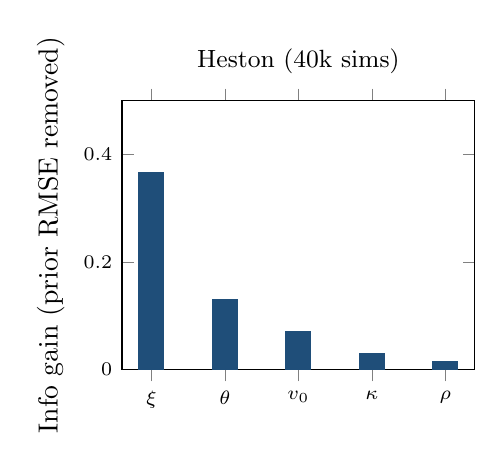
\begin{tikzpicture}
\begin{axis}[width=0.5\textwidth, height=5cm, ybar, bar width=9pt,
  symbolic x coords={$\xi$, $\theta$, $v_0$, $\kappa$, $\rho$},
  xtick=data, ymin=0, ymax=0.5,
  ylabel={Info gain (prior RMSE removed)},
  tick label style={font=\scriptsize},
  title={\small Heston (40k sims)}]
\addplot[fill=npblue, draw=npblue] coordinates
  {($\xi$,0.365) ($\theta$,0.13) ($v_0$,0.07) ($\kappa$,0.03)
   ($\rho$,0.015)};
\end{axis}
\end{tikzpicture}\hfill
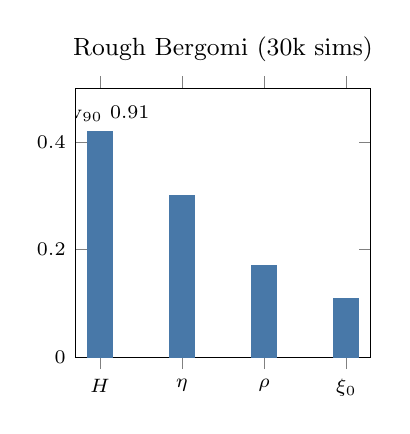
\begin{tikzpicture}
\begin{axis}[width=0.44\textwidth, height=5cm, ybar, bar width=9pt,
  symbolic x coords={$H$, $\eta$, $\rho$, $\xi_0$},
  xtick=data, ymin=0, ymax=0.5,
  tick label style={font=\scriptsize},
  title={\small Rough Bergomi (30k sims)}]
\addplot[fill=npmid, draw=npmid] coordinates
  {($H$,0.42) ($\eta$,0.30) ($\rho$,0.17) ($\xi_0$,0.11)};
\node[font=\scriptsize, anchor=south] at (axis cs:$H$,0.42)
  {cov$_{90}$ 0.91};
\end{axis}
\end{tikzpicture}
\caption{Likelihood-free calibration: information gain (fraction of
prior RMSE removed by one 252-day path) per parameter, Heston (left,
$\kappa$/$\rho$ at midpoints of their reported weak ranges) and rough
Bergomi (right). Honesty check by SBC coverage: Heston cov$_{90}$
0.85--0.90 across all five parameters; rough Bergomi 0.85--0.92, with
the Hurst roughness $H$ at 0.91 --- informative \emph{and} calibrated.}
\label{fig:sbc}
\end{figure}

\textbf{Heston.} From 40k simulated (parameter, 252-day path) pairs and
ten path summaries, the amortized posterior is calibrated (central
coverage cov$_{80}$ 0.78--0.80, cov$_{90}$ 0.85--0.90 for all five
parameters) and informative where a single path identifies:
vol-of-vol info-gain 36.5\% (fraction of prior RMSE removed), long-run
variance 13\%, with mean-reversion and leverage weakly identified ---
the honest, expected pattern.

\textbf{Rough Bergomi (the marquee result).} The rough-volatility model
\citep{bayer2016rbergomi, gatheral2018roughvol} --- volatility whose path
is driven by fractional noise controlled by the Hurst exponent $H$, with
$H<0.5$ producing paths jaggier than any standard model allows ---
has a non-Markovian fractional driver and no tractable likelihood;
neither MLE nor any GARCH-family filter can fit it. The amortized
posterior over $(H, \eta, \rho, \xi_0)$ from a single 252-day path (30k
sims) \textbf{recovers the Hurst roughness $H$ with info-gain 0.42 and
SBC cov$_{90}$ 0.91} (IQN; GBM 0.89); $\eta$ info-gain 0.30; all
coverages 0.85--0.92. Recovering the parameter that \emph{defines} rough
volatility --- notoriously difficult classically --- with calibrated
uncertainty from one path is, we believe, the strongest demonstration to
date that GBC does something structurally new in finance. Here the
neural IQN is not merely competitive but canonical: it is the estimator
that \emph{samples} the posterior; trees provide fixed quantiles only.


%% ===== HONEST UNCERTAINTY ON THE RISK NUMBER =====
\section{Honest uncertainty on the risk number}\label{sec:uncertainty}

\noindent\emph{Conclusion of this section, stated first.} The deployable
uncertainty on the risk number is delivered by the block bootstrap and an
EVT tail, both on GARCH-standardized residuals; the Gibbs
generalized-Bayes posterior is retained here \emph{only as a diagnostic}.
Its loss exponent treats observations as independent, so on financial
data --- where volatility clustering makes the effective sample size far
below $n$ --- it is overconfident by a factor of $1.6$ on raw returns.
Residual space repairs the honesty, but at that point the Gibbs machinery
adds little beyond the bootstrap it must be calibrated against; we
therefore present it as evidence of the dependence problem, not as a
recommended tool. This is the paper's answer to the standing question of
whether generalized Bayes is usable for a financial risk number: not on
its own terms.

\medskip
Every model so far outputs a \emph{point} VaR/ES. None tells the desk
how uncertain that number is. This section delivers calibrated
uncertainty bands on $(\VaR,\ES)$ and, on the way, settles a
methodological question: whether the Gibbs-posterior program of
generalized Bayes \citep{jiang2008gibbs, bissiri2016general} --- a
posterior over the risk functional built from the loss itself --- is
usable on financial data at all. Its guarantees assume
near-independence; financial returns are anything but. The answer, in
numbers: not on raw returns (a factor-1.6 overconfidence we measure
directly), yes after GARCH filtering --- but the workhorses of the
calibrated construction turn out to be the block bootstrap (resampling
contiguous blocks of days, not single days, so the resample preserves
serial dependence) \citep{kunsch1989block}, adaptive conformal
inference\footnote{ACI \citep{gibbs2021aci} treats miscoverage as a
control problem: after each day the working level is nudged,
$\alpha_{t+1} = \alpha_t + \gamma(\alpha - \mathbb{I}\{\text{breach at }
t\})$, so a run of breaches automatically widens the band and a
breach-free run relaxes it --- split conformal's guarantee made robust
to distribution drift, at the cost of targeting long-run rather than
conditional coverage.}, and an extreme-value tail interval, with the
repaired Gibbs posterior as a supporting variant rather than the
centerpiece. One further generalized-Bayes result deserves record: in
the project's pre-registered daily single-portfolio study --- the honest
anchor in which a leverage-aware GARCH was the best standalone model and
the standalone network only reached parity --- a Gibbs-posterior model
\emph{average} that included the network did best of all. Loss-based
posterior weighting earns its keep as an ensembling device even where
the standalone generative model does not win.

\subsection{The defect, measured}

On 80 CRSP names at $\tau = 0.05$, we compare the Gibbs posterior SD of
the VaR level to the true sampling SD estimated by moving-block
bootstrap (block 20). On \emph{raw returns}: Gibbs SD 0.108 vs block SD
0.179 --- the naive posterior understates VaR uncertainty by a factor
$R = 1.64$ (median 1.59). The i.i.d.-bootstrap ratio is 1.19, so the
1.19$\to$1.64 gap isolates the serial-dependence contribution: vol
clustering makes the effective sample size far smaller than $n$, and the
product-form posterior over-concentrates accordingly.

\subsection{The repair: residual space}

The identical construction on GARCH-standardized residuals gives $R =
0.79$: the overconfidence is gone (mildly conservative, the safe
direction). The mechanism is confirmed independently: on residuals,
block and i.i.d.\ bootstraps agree (VaR coverage 0.947 vs 0.953 at
$\alpha=2.5\%$) --- the filter has absorbed the dependence, restoring
the i.i.d.-like regime in which loss-based posteriors are honest. This
is the same scale/shape division of labor as the residual-hybrid, now
applied to \emph{uncertainty} rather than accuracy. An adaptive conformal
arm \citep{gibbs2021aci} corroborates from the coverage side: ACI attains
the best and most stable realized VaR coverage under drift (5.03\%
realized at the 5\% level; rolling max-deviation 0.042, vs 0.059 GARCH
and 0.074 for a fixed empirical window). A complementary, benchmark-free
reliability signal comes from ensemble disagreement: the dispersion of
quantile forecasts across independently trained networks correlates
$+0.11$ with the model's own realized error --- crude, but free, and
usable as a first-line screen ahead of the formal bands of
Section~\ref{sec:bands}.

\subsection{Calibrated credible bands on $(\VaR, \ES)$}\label{sec:bands}

\begin{table}[t]
\centering
\begin{threeparttable}
\caption{Coverage of nominal-90\% credible/confidence bands for the
residual $(\VaR,\ES)$, 150 CRSP names.}
\label{tab:bands}
\begin{tabular}{lcccc}
\toprule
& \multicolumn{2}{c}{$\VaR$} & \multicolumn{2}{c}{$\ES$} \\
\cmidrule(lr){2-3}\cmidrule(lr){4-5}
Method & $\alpha=1\%$ & $\alpha=2.5\%$ & $\alpha=1\%$ & $\alpha=2.5\%$ \\
\midrule
Block bootstrap (residuals) & 0.947 & 0.953 & 0.86 & \textbf{0.90} \\
i.i.d.\ bootstrap (residuals) & 0.96 & 0.947 & --- & --- \\
Gibbs, naive $\omega=1$ & 0.987--0.993 & (over-wide) & --- & --- \\
Gibbs, $\omega$-calibrated & \textbf{0.953--0.967} & & --- & --- \\
EVT/GPD ES interval & --- & --- & \textbf{0.887} & \textbf{0.90} \\
\bottomrule
\end{tabular}
\begin{tablenotes}\footnotesize
\item Reading guide --- two different probability levels appear here,
do not conflate them: $\alpha$ is the \emph{risk level} of the quantile
being estimated ($\VaR$ at 1\% or 2.5\%); each entry is the realized
\emph{coverage of the nominal-90\% uncertainty band} around that risk
number, i.e., the fraction of experiments in which the band contained
the truth. Ideal is exactly 0.90: above 0.90 means the band is
wastefully wide (over-conservative), below means overconfident. Bold
marks the entry closest to 0.90 in each column --- so the calibrated
Gibbs (0.953--0.967) \emph{beats} the naive one (0.987--0.993), whose
larger numbers look reassuring but signal over-wide bands. The
naive-$\omega$ Gibbs over-covers because pinball
is shallow in the sparse tail; matching the posterior SD to the block
SD repairs it. The 99\% ES block interval under-covers (0.86, too few
tail points); the GPD interval reaches 0.887 at the honest price of
width (2.12 vs 1.31).
\end{tablenotes}
\end{threeparttable}
\end{table}

\begin{figure}[t]
\centering
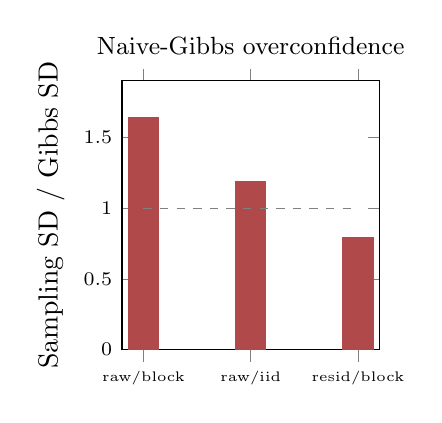
\begin{tikzpicture}
\begin{axis}[width=0.4\textwidth, height=5cm, ybar, bar width=11pt,
  symbolic x coords={raw/block, raw/iid, resid/block},
  xtick=data, ymin=0, ymax=1.9,
  ylabel={Sampling SD / Gibbs SD},
  x tick label style={font=\tiny}, tick label style={font=\scriptsize},
  title={\small Naive-Gibbs overconfidence}]
\addplot[fill=gred, draw=gred] coordinates
  {(raw/block,1.64) (raw/iid,1.19) (resid/block,0.79)};
\addplot[dashed, gray, sharp plot] coordinates
  {(raw/block,1) (resid/block,1)};
\end{axis}
\end{tikzpicture}\hfill
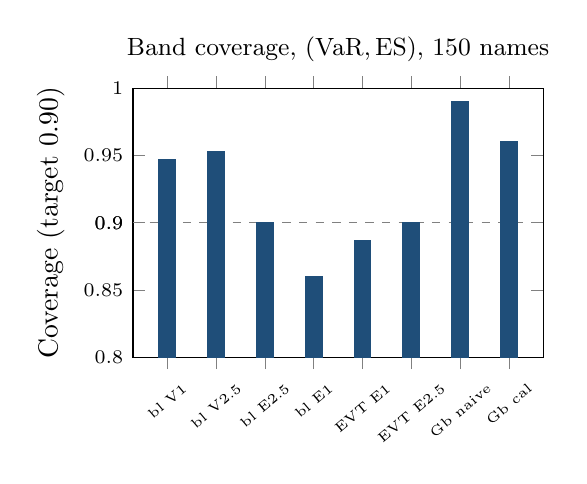
\begin{tikzpicture}
\begin{axis}[width=0.56\textwidth, height=5cm, ybar, bar width=6pt,
  symbolic x coords={bl V1, bl V2.5, bl E2.5, bl E1, EVT E1, EVT E2.5,
                     Gb naive, Gb cal},
  xtick=data, ymin=0.8, ymax=1.0,
  ylabel={Coverage (target 0.90)},
  x tick label style={font=\tiny, rotate=40},
  tick label style={font=\scriptsize},
  extra y ticks={0.9},
  extra y tick style={grid=major, grid style={dashed, gray}},
  title={\small Band coverage, $(\VaR,\ES)$, 150 names}]
\addplot[fill=npblue, draw=npblue] coordinates
  {(bl V1,0.947) (bl V2.5,0.953) (bl E2.5,0.90) (bl E1,0.86)
   (EVT E1,0.887) (EVT E2.5,0.90) (Gb naive,0.99) (Gb cal,0.96)};
\end{axis}
\end{tikzpicture}
\caption{Honest uncertainty, assembled. Left: the naive Gibbs posterior
SD understates the block-bootstrap sampling SD $1.64\times$ on raw
returns (i.i.d.\ bootstrap 1.19 --- the gap is the dependence
contribution); the ratio falls to 0.79 on GARCH residuals. Right:
coverage of nominal-90\% bands (bl $=$ block bootstrap; V $=$ VaR, E $=$
ES at the stated level; Gb $=$ Gibbs, naive $\omega$ vs
$\omega$-calibrated). Block bootstrap and the EVT interval sit at or
near target; the naive Gibbs over-covers.}
\label{fig:bands}
\end{figure}

Table~\ref{tab:bands} assembles the end-to-end result: block bootstrap
on residuals for VaR and 2.5\% ES; the $\omega$-calibrated Gibbs
posterior as the parametric credible band; EVT for the deep ES tail ---
every piece at or near nominal. To our knowledge no standard risk model
(GARCH, CAViaR, FHS, or our own hybrid) supplies any counterpart. Two
refinements remain registered: the loss-in-the-exponent ablation (CRPS,
tail-CRPS, the Fissler--Ziegel joint $(\VaR,\ES)$ score
\citep{fissler2016}, MEU) and formal comparison of $\omega$-calibration
to SafeBayes-style procedures \citep{grunwald2017safebayes}.


%% ===== THE MULTIVARIATE TAIL: HONEST NEGATIVE =====
\section{The multivariate tail: negatives, then a crossover}
\label{sec:multivariate}

We report the negatives first, because they discipline the claim. Three
direct nonparametric attacks on the portfolio tail all lose to
multivariate GARCH: (i) a direct pooled portfolio-quantile model on a
diversified 25-name basket \citep[DCC/CCC --- multivariate GARCH with
dynamic (DCC) or constant (CCC) correlations across assets ---
benchmarks
after][]{engle2002dcc} (DCC 0.1709 $<$ CCC 0.1719 $<$ GBM 0.1752,
ordering preserved in the crisis decile); (ii) a concentration sweep
($K = 2,\dots,25$ by pairwise correlation) --- the gap does not close as
the basket concentrates; (iii) a neural weight-input IQN
$Q(\tau \mid s, w)$ trained across the simplex --- roughly $2\times$
worse than CCC/DCC at every weighting, because a network fed summary
state never recovers the quadratic form $w'\Sigma w$ that GARCH models
explicitly. The covariance \emph{is} the object; we concede equity
co-crash to explicit covariance models.

\begin{figure}[t]
\centering
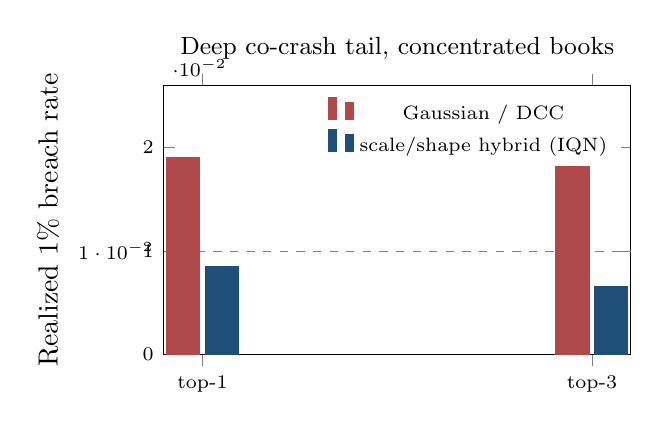
\begin{tikzpicture}
\begin{axis}[width=0.62\textwidth, height=5cm, ybar, bar width=12pt,
  symbolic x coords={top-1, top-3},
  xtick=data, ymin=0, ymax=0.026,
  ylabel={Realized 1\% breach rate},
  tick label style={font=\scriptsize},
  extra y ticks={0.01},
  extra y tick style={grid=major, grid style={dashed, gray}},
  legend style={font=\scriptsize, draw=none, at={(0.98,0.98)},
                anchor=north east},
  title={\small Deep co-crash tail, concentrated books}]
\addplot[fill=gred, draw=gred] coordinates
  {(top-1,0.019) (top-3,0.0185)};
\addlegendentry{Gaussian / DCC}
\addplot[fill=npblue, draw=npblue] coordinates
  {(top-1,0.0085) (top-3,0.0066)};
\addlegendentry{scale/shape hybrid (IQN)}
\end{axis}
\end{tikzpicture}
\caption{The deep-tail crossover on the most concentrated weighting
schemes (top-1 and top-3 books; Gaussian/DCC top-3 drawn at the midpoint
of its reported 0.018--0.019). Across \emph{all} schemes Gaussian/DCC
realizes 0.018--0.024 --- roughly twice the nominal 0.01 --- while the
covariance-scale / nonparametric-shape hybrid is near or under target.
At the moderate 5\% tail the ordering reverses.}
\label{fig:cocrash}
\end{figure}

The rescue is, once again, the hybrid division of labor: DCC supplies
the portfolio scale $\sigma_{w,t}$; a generative IQN learns only the
shape of the standardized portfolio residual, conditioned on
concentration (the Herfindahl index: the sum of squared portfolio
weights, higher meaning more concentrated), state, and weights.
Calibration is restored
(PIT-KS 0.30 $\to$ 0.055--0.075 --- a Kolmogorov--Smirnov test of
whether probability-integral-transformed outcomes look uniform, i.e.\
whether the model is calibrated --- comparable to Gaussian/DCC), and a
clean crossover emerges: Gaussian/DCC is adequate at the moderate 5\%
tail (where the IQN is slightly conservative) but systematically
\emph{thin} in the deep 1\% tail (cov$_{01}$ 0.018--0.024, roughly twice
nominal breaches), while the hybrid is near nominal everywhere and best
precisely on concentrated books (top-1 concentration: cov$_{01}$ 0.0085
vs target 0.01; Gaussian 0.019). The multivariate contribution is thus
representational and calibrational: a samplable joint downside law whose
deep co-crash tail is honest where the industry model's is thin ---
reported alongside, not instead of, the three negatives.


%% ===== CONCLUSION (skeleton) =====
\section{Conclusion}\label{sec:conclusion}
%% TODO: write. Thesis: amortized/likelihood-free quantile inference
%% is calibrated for intractable univariate stochastic-vol models
%% (rough vol especially) but fails honestly on real multivariate tails.

%% ===== BIBLIOGRAPHY =====
\bibliographystyle{plainnat}
\bibliography{refs_v3}

\appendix
%% ===== PROOF: generative sampler =====
\section{Proof}\label{app:proofs}
\subsection*{Proof of Lemma~\ref{lem:sampler} (generative sampler)}

Let $\widetilde q(\cdot\mid s):(0,1)\to\mathbb{R}$ be nondecreasing and
left-continuous, $\tau\sim U(0,1)$, and $Z^*=\widetilde q(\tau\mid s)$.
Fix $x\in\mathbb{R}$ and put $G(x)=\sup\{t\in(0,1):\widetilde q(t\mid
s)\le x\}$ (with $\sup\varnothing=0$). Because $\widetilde q$ is
nondecreasing, $\{t:\widetilde q(t\mid s)\le x\}$ is an initial
subinterval of $(0,1)$; left-continuity of $\widetilde q$ makes the
supremum attained, so the set is $(0,G(x)]$ and
\[
\{\widetilde q(\tau\mid s)\le x\}=\{\tau\le G(x)\}.
\]
Since $\tau\sim U(0,1)$, $\Pr(Z^*\le x)=\Pr(\tau\le G(x))=G(x)$; thus
$Z^*$ has cumulative distribution function $G$, the generalized inverse
of $\widetilde q$. For a nondecreasing left-continuous $\widetilde q$
the generalized inverse of its generalized inverse recovers the
original function, so the quantile function of $Z^*$ is exactly
$\widetilde q(\cdot\mid s)$. \hfill$\square$

% FORMAT NOTE: finance/econometrics venues use single-column,
% author-year (natbib) format -- NOT IEEE. This file is standard
% working-paper/SSRN format and ports directly:
%  - J. Financial Econometrics: OUP template ('Modern Small'), <=40
%    double-spaced pages, ORCID required, data/code sharing encouraged.
%  - J. Banking & Finance / JFE-family: Elsevier elsarticle class,
%    Harvard author-year.
%  - Quantitative Finance: Taylor & Francis interact class.
%  - Bayesian Analysis (Paper-B split): ba class, natbib.
% Keep booktabs tables, no vertical rules, author-year cites throughout.


%% ===== GLOSSARY (shared; trim to B-relevant entries) =====
\section{Glossary}\label{app:glossary}

Written so that a reader from any one field can parse every other
field's terms. Formulas referenced are in Section~\ref{sec:methods}.

\begin{description}[leftmargin=1.6em,itemsep=1pt,font=\normalfont\bfseries]
\item[VaR / ES] Value-at-Risk: the loss threshold exceeded with
probability $\tau$ (a quantile with the sign flipped); Expected
Shortfall: the average loss \emph{given} VaR is exceeded
(\S\ref{sec:notation}). FRTB capitalizes ES at $\tau=2.5\%$.
\item[Pinball (check) loss] The asymmetric absolute loss
\eqref{eq:pinball} whose minimizer is the true quantile; the strictly
proper score for quantile forecasts. Reported edges (``$+2.7\%$ of
pinball'') are percentage reductions in this loss.
\item[GARCH-$t$ / GJR / EWMA] Parametric filters for conditional
variance \eqref{eq:garch}; GJR adds a leverage term (down-moves raise
vol more); EWMA is the fixed-decay special case (RiskMetrics);
Student-$t$ fixes the innovation shape.
\item[HS / FHS] Historical simulation: empirical quantiles of past
returns. Filtered HS: empirical quantiles of GARCH-standardized
residuals, rescaled by today's $\widehat\sigma_t$ --- the regulatory
workhorse; the special case of \eqref{eq:hybrid} with no state
dependence.
\item[CAViaR] Conditional autoregressive VaR: models the quantile
itself as an autoregression, estimated on the pinball loss; the one
non-nested rival.
\item[EVT / GPD / POT] Extreme-value theory: exceedances over a high
threshold converge to the generalized Pareto distribution; fitting it
(peaks-over-threshold) gives the tail extrapolation \eqref{eq:evt}.
\item[Conformal prediction] Distribution-free finite-sample correction
sized on a held-out split (Proposition~\ref{prop:conformal}); guarantees
coverage under exchangeability without any distributional assumption.
\item[Quantile regression / IQN] Estimating conditional quantiles by
pinball ERM; the implicit quantile network \eqref{eq:iqn} takes the
level $\tau$ as an \emph{input}, so one network carries the whole
distribution and sampling is evaluation at random $\tau$.
\item[GBM (trees)] Gradient-boosted regression trees on the pinball
loss; the strongest point estimator on tabular features; cannot sample.
\item[Amortization] Training one model across many assets so inference
for a new asset is evaluation, not estimation; the generative-Bayes
reading is the inverse map $z \overset{D}{=} H(s,\tau)$
(\S\ref{sec:gbcmethod}).
\item[Gibbs / generalized-Bayes posterior] A posterior built from a
loss instead of a likelihood, \eqref{eq:gibbs}; $\omega$ tempers how
fast the loss overwhelms the prior.
\item[SBC] Simulation-based calibration: simulate known truths, check
the posterior's ranks are uniform; the audit in Algorithm 3.
\item[Walk-forward, purge, embargo] Refit on past data only, on a
schedule; delete observations adjacent to the train/test boundary so
overlapping windows cannot leak information.
\item[DM test] Diebold--Mariano: a $t$-test on the loss difference
between two forecasters, robust to serial correlation.
\item[MCS] Model Confidence Set: the subset of models not
statistically dominated at a given level --- ``co-best'' means surviving
in that set.
\item[Kupiec / Christoffersen] Regulatory exception tests: correct
\emph{number} of VaR breaches (unconditional coverage) and breaches
arriving \emph{independently} rather than in clusters.
\item[DCC] Dynamic conditional correlation: the standard multivariate
GARCH benchmark for portfolio tails.
\item[VRP; $\PP$ vs.\ $\Q$] Variance risk premium: option-implied
variance exceeds realized on average. $\PP$ is the physical measure
(what happens); $\Q$ the risk-neutral measure (what option prices
imply); their wedge at the put wing is the crash premium studied in the
companion paper.
\item[Misspecification frontier] The trailing residual-shape score
\eqref{eq:score} and the empirical fact that the nonparametric edge
concentrates in its top decile.
\end{description}


\end{document}
